\documentclass[12pt]{article}

\usepackage[dvips,letterpaper,margin=0.75in,bottom=0.75in]{geometry}
\usepackage{cite}
\usepackage{slashed}
\usepackage{graphicx}
\usepackage{amsmath}
\usepackage{braket}
\usepackage{latexsym,amssymb,amsmath}

\usepackage[american,fulldiode]{circuitikz}
\tikzset{component/.style={draw,thick,circle,fill=white,minimum size =0.75cm,inner sep=0pt}}

\begin{document}
\ctikzset{bipoles/thickness=1}
\ctikzset{bipoles/length=.6cm}

\title{Review of Cold Electronics}
\author{Michael Mulhearn}

\maketitle

\section{Survey of Relevant Devices}

\begin{tabular}{lccc}
Device & Technology & Institution & Reference \\
DUNE Front-end ASIC & 180 nm CMOS & BNL & \cite{bnl-dune-afe}\\
SCT Front-end ASIC & 250 nm CMOS & BNL & \cite{bnl-telescope}\\
MicroBooNE Front-End ASIC & 180 nm CMOS & BNL & \\
\end{tabular}


%\section{Overview of Challenges}
%The requirements on the readout for the DUNE front-end cold ASIC include:
%\begin{itemize}
% \item $300~\rm fC$ charge readout with resolution better than 1000 rms electrons.
 %\item 12-bit resolution
% \item Readout at 2 MS/s
 %\item Maximum 10 mW per channel.
%\end{itemize}

%\section{People}
%\begin{itemize}
%\item Cressler 
%\item V.~Radeka 
%\item Geronimo
%\end{itemize}

\section{Transistor Modelling}


\begin{figure}[htbp]
\begin{center}
\begin{circuitikz}[line width=1pt]
\draw (0,0) node[nmos](nmosa){};
\draw (nmosa.G) to[resistor,l=$R_{\rm s}$] ++(-1.0,0);
\end{circuitikz} 
\caption{Model for intrinsic thermal noise as Johnson-Nyquist noise from an equivalent series resistance $R_{\rm S}$.}
\label{fig:encmodel}
\end{center}
\end{figure}

For a well-designed amplifier based on a field-effect transistor, the noise will be dominated by the intrinsic thermal noise in the conducting channel, so that the drain current spectral density is given by
\begin{displaymath}
\braket{i_{\rm D}^2} = 4 k T a_n g_m
\end{displaymath}
where $a_n$ is a dimensionless constant.  Because the drain current and gate voltage are related by the transconductance:
\begin{displaymath}
i_{\rm D} = g_{\rm m} v_{\rm G}
\end{displaymath}
we can interpret the spectral density as if it were due to Johnson-Nyquist noise of an equivalent resistance $R_{\rm s}$ in series with the gate terminal:
\begin{displaymath}
\braket{v_{G}^2} = 4 k T R_{\rm s}
\end{displaymath}
with 
\begin{displaymath}
R_{\rm s} = a_n / g_m
\end{displaymath}
For field effect devices $a_n \sim 2/3$.

The equivalent noise charge is the voltage spectral density multiplied by an effective bandwidth $1/t_{\rm m}$ from the impulse response of the amplifier, and scaled by the input capacitance $C_{\rm in}$:
\begin{displaymath}
ENC^2 = 4 k T R_{\rm s} C^2_{\rm in} \frac{1}{t_m}
\end{displaymath}

The explicit temperature dependence is favorable to operation of a front-end amplifier under cryogenic conditions, but for precise modeling, the temperature dependence of the transistor parameters must also be understood.

\section{Lifetime Reliability}

The lifetime reliability of CMOS devices is degraded by four major effects:  electromigration (EM), stress migration, thermal cycling (TC), and hot-carrier effects.

Electromigration (EM) is the movement of the conductor atoms from collisions with conducting electrons, which results in degradation of interconnects.  The mean time to failure (MTTF) is:
\begin{displaymath}
{\rm MTTF}_{\rm EM} \propto J^{-n} \, \exp\left( \frac{E_{\rm EM}}{k_{\rm b}T}\right)
\end{displaymath}
where $J$ is the current density in the interconnect, $E_{\rm EM}$ is the activation energy for electromigration, and $n$ is a constant for the conductor material.  For copper $E_{\rm EM} = 1.1~\rm eV$ and $n=0.9$.  

Stress migration (SM) is the movement of conductor ions under thermo-mechanical stress resulting from mismatched thermal expansion rates, which results in degradation of interconnects.  The mean time to failure is:
\begin{displaymath}
{\rm MTTF}_{\rm SM} \propto  |T_0 - T|^{-m} \, \exp\left( \frac{E_{\rm SM}}{k_{\rm b}T}\right)
\end{displaymath}
where $T_0$ is the metal deposition temperature, and $m$ and $E_{\rm SM}$ are material properties.  For copper, $E_{\rm SM} = 0.9~\rm eV$ and $n=2.5$.

Thermal cycling (TC) is alternating heating and cooling of the device causing the accumulation of permanent mechanical damage.
\begin{displaymath}
{\rm MTTF}_{\rm TC} \propto \left( \frac{1}{\Delta T}\right)^q
\end{displaymath}
Where $\Delta T$ is the change in temperature during one thermal cycle and $q$ is an empirical constant for the material.  

Under cryogenic conditions, the exponential dependence on temperature ensures that the effect of electromigration and stress migration on lifetime becomes neglible.  Likewise, if held under constant cryogenic conditions, $\Delta T \to 0$ and so the effect of thermal cycling is likewise negligible.

\begin{figure}[htbp]
\begin{center}
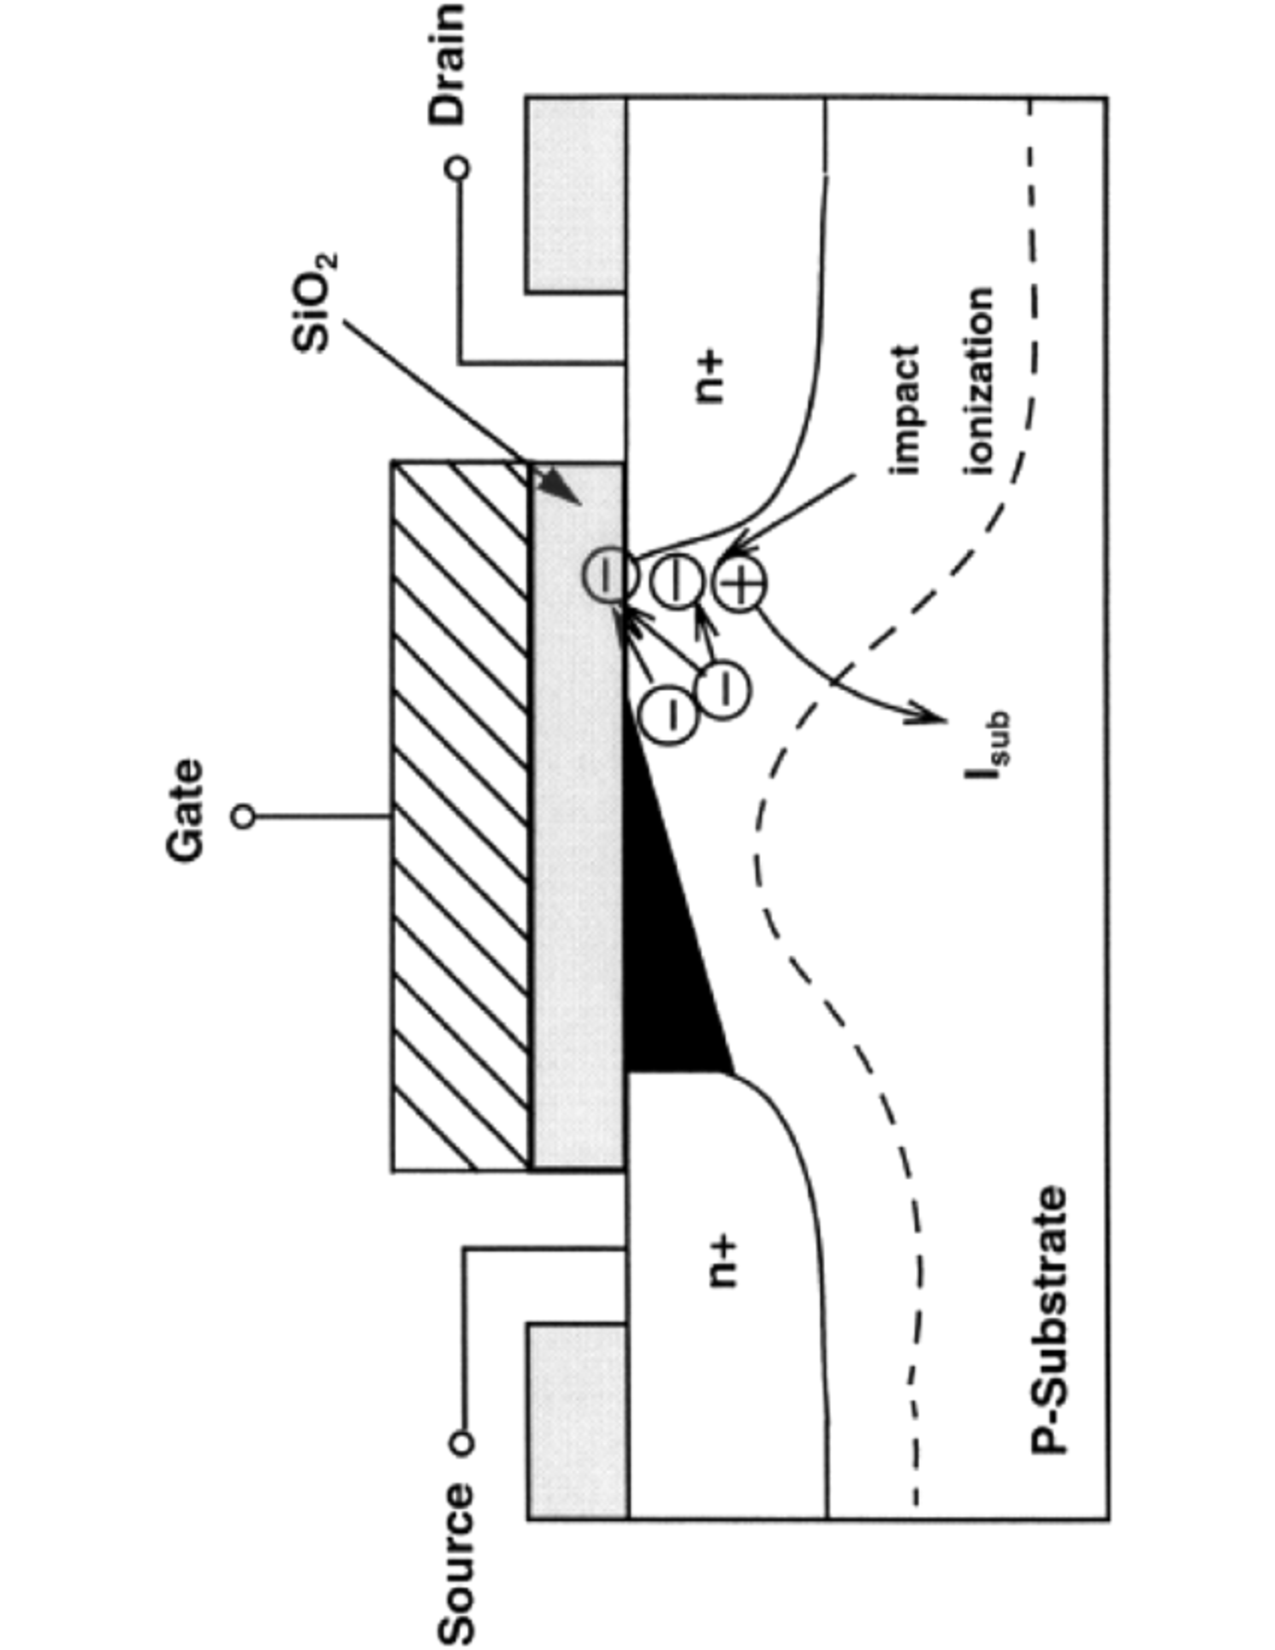
\includegraphics[width=0.45\textwidth,angle=270]{figs/hot-carrier.pdf} 
\caption{Schematic for interface state creation by hot-electrons, from \cite{hot-carrier-effects}.}
\label{fig:lifetime}
\end{center}
\end{figure}

That leaves hot-carrier effects, which we consider in the lucky-electron model.   To reach sufficient energy $\phi_i \sim 1.3~\rm eV$ to create an electron-hole pair, an electron accelerated by an electric field $E_{\rm m}$ must travel at least a distance:
\begin{displaymath}
d = \frac{\phi_i}{q E_{\rm m}}
\end{displaymath}
If the mean free path of the electron is $\lambda$, than the probability of an electron creating an electron-hole pair is:
\begin{displaymath}
\exp\left(-\frac{\phi_i}{q \lambda E_{\rm}}\right)
\end{displaymath}
Such an electron is called hot by analogy to a thermodynamic Boltzman factor.

In the context of a MOSFET, $E_m$ is the difference between the applied voltage $V_{\rm ds}$ and the pinch off voltage.  Hot electrons, and the electron hole pairs they produce, will be produced predominantly near the drain.  The electrons will simply contribute to $I_{\rm ds}$, but the holes drift into the substrate, producing a substrate current:
\begin{equation}\label{eqn:isub}
I_{\rm sub} = C_1 I_{\rm ds} \exp\left(-\frac{\phi_i}{q \lambda E_{\rm}}\right)
\end{equation}
The substrate current is proportional to the rate of hot-carrier creation and is therefore serves as a monitor for all hot-carrier effects.

\begin{figure}[htbp]
\begin{center}
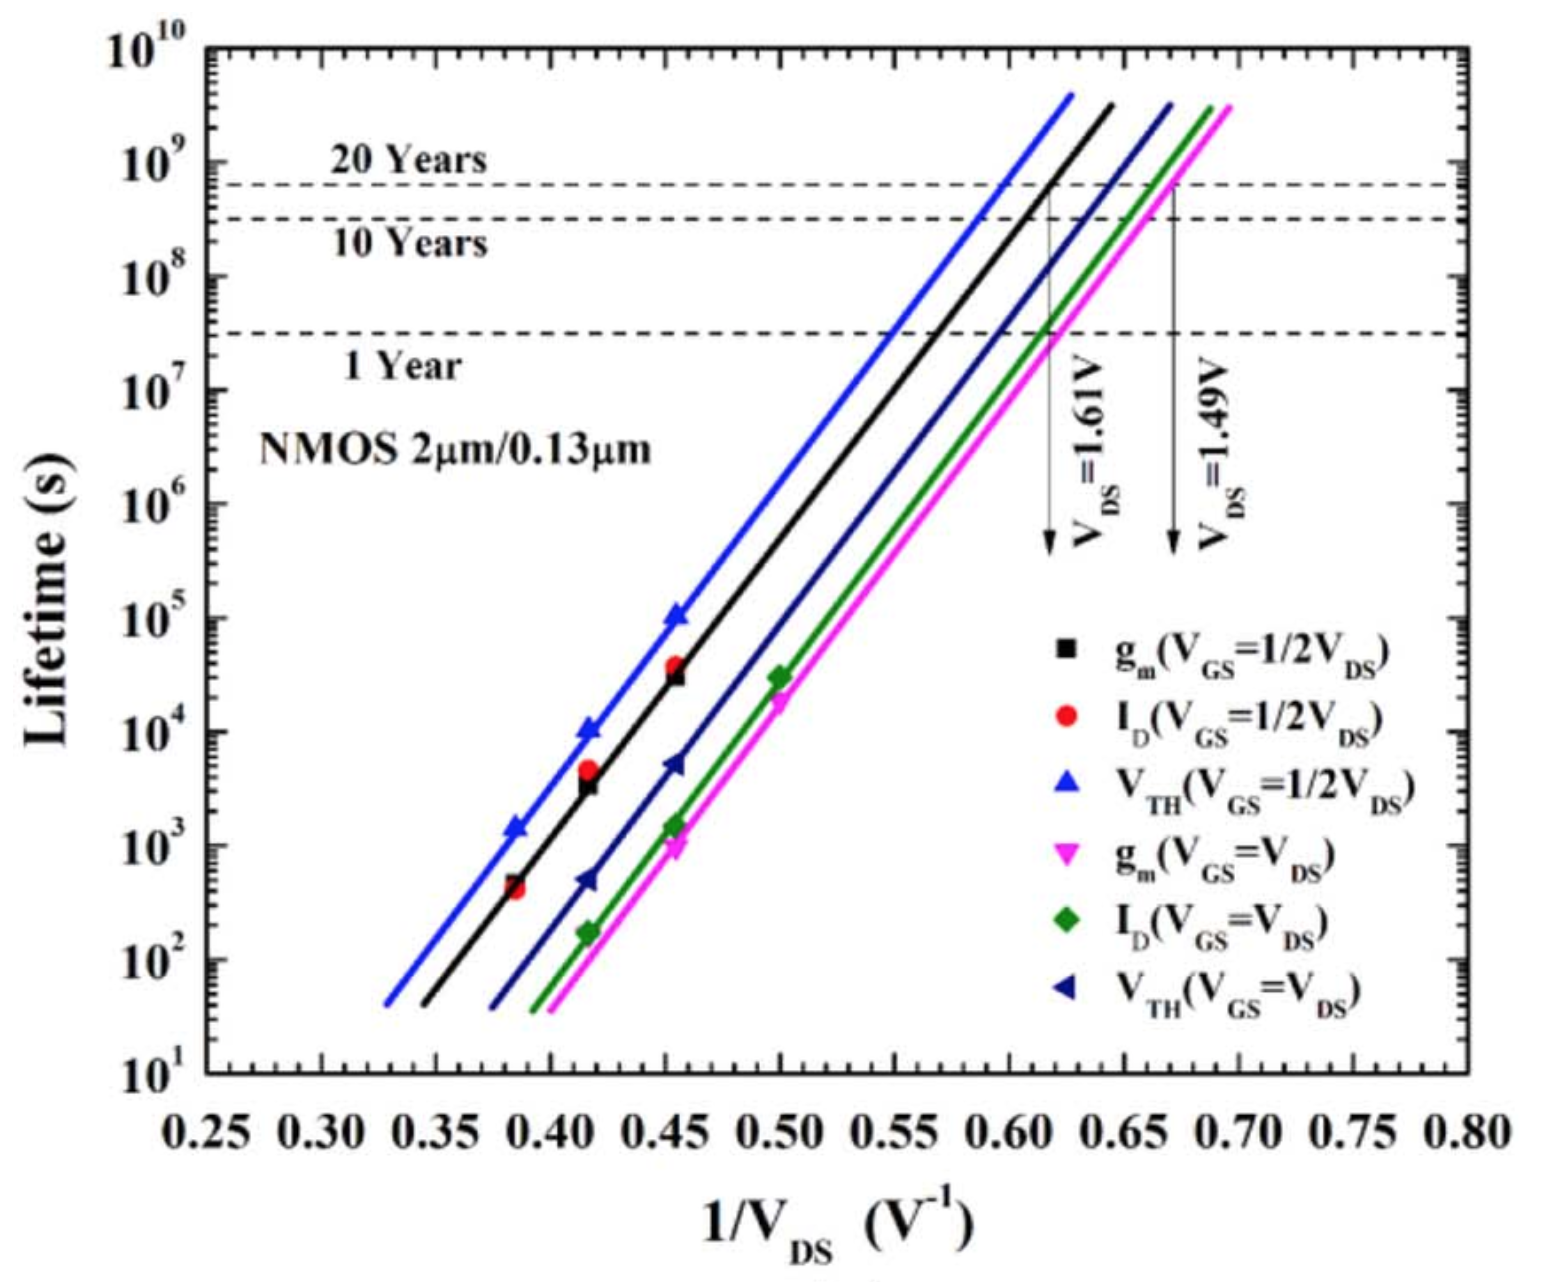
\includegraphics[width=0.55\textwidth]{figs/lifetime_vstress.png} 
\caption{Example of over-voltage stress-testing to determine lifetime from \cite{hot-carrier-effects}.}
\label{fig:lifetime}
\end{center}
\end{figure}

Hot-carriers that reach sufficient energy $\phi_{\rm it} \sim 3.7~\rm eV$can create an interface state (acceptor-like trap) in the $\rm Si-SiO_2$ interface.  This degrade transistor parameters such as transconductance, input resistance, and threshold voltage.  Such hot-carriers are produced at a rate per channel width $W$ proportional to:
\begin{displaymath}
\frac{I_{\rm ds}}{W} \exp\left(-\frac{\phi_{\rm it}}{q \lambda E_{\rm}}\right)
\end{displaymath}
and so we can expect the lifetime (defined as some well-defined degradation in a particular parameter)
to be:
\begin{equation}\label{eqn:tau}
\tau = C_2 \frac{W}{I_{\rm ds}}\exp\left(\frac{\phi_{\rm it}}{q \lambda E_{\rm}}\right)
\end{equation}
From which we notice: 
\begin{displaymath}
\log(\tau) \propto \frac{1}{\lambda E_{\rm m}}
\end{displaymath}
Since the mean free path increases as the temperature decreases, hot-carrier effects can significantly reduce the lifetime of CMOS sensors in cryogenic conditions, and therefore must be estimated for each CMOS technology.  Since $E_m$ is related to the applied voltage, a popular approach is to raise $V_{\rm ds}$ until the lifetime is short enough to conveniently measure, then extrapolate back to the intended value for $V_{\rm ds}$.  An example is shown in Fig.~\ref{fig:lifetime}.

\begin{figure}[htbp]
\begin{center}
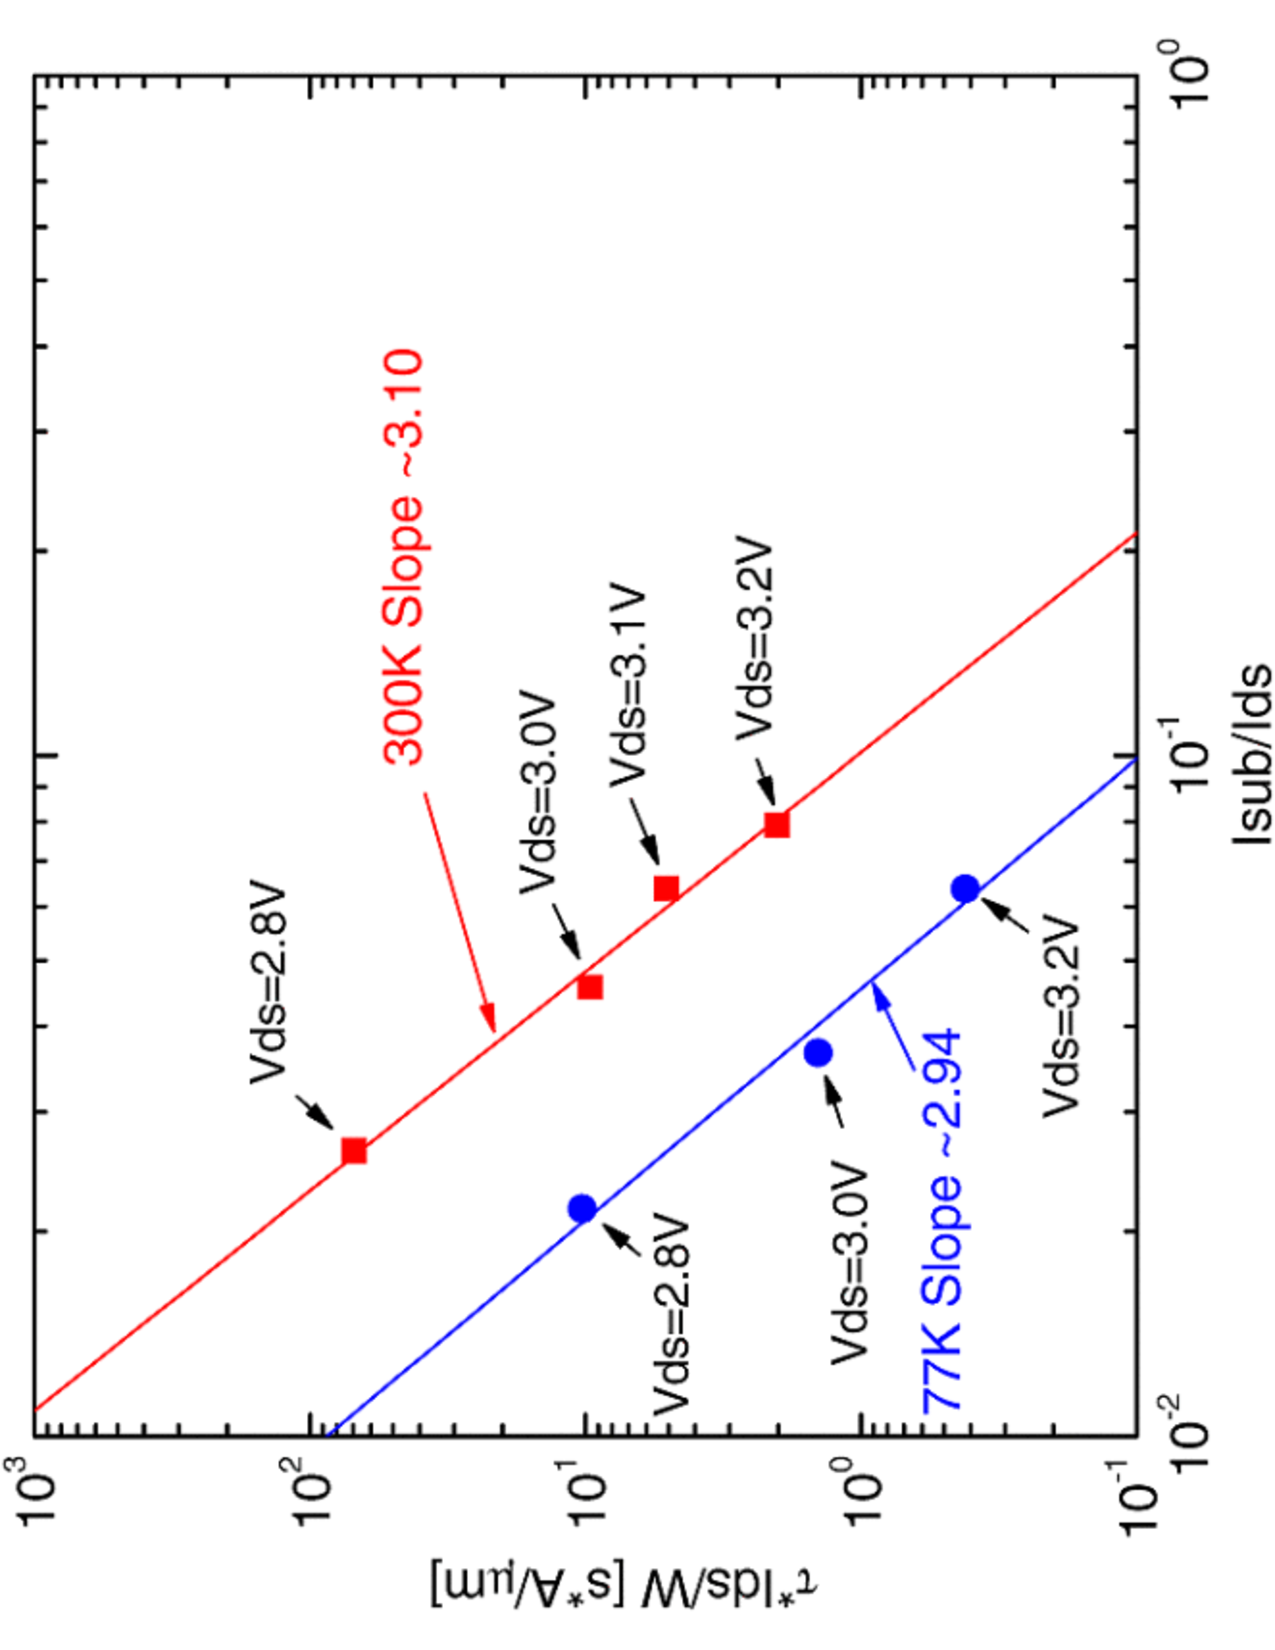
\includegraphics[width=0.45\textwidth,angle=270]{figs/lifetime_isub.pdf} 
\caption{Example showing expected power-law relationship between $I_{rm sum}/I_{\rm ds}$ and $\tau I_{\rm ds}/W$, with slope $\phi_{\rm it}/\phi_{i} \sim 3$.  From \cite{hot-carrier-effects}.}
\label{fig:lifetime}
\end{center}
\end{figure}

Another approach comes from Combining Equations ~\ref{eqn:isub} and \ref{eqn:tau} to eliminate the factor $q \lambda E_{\rm}$ to obtain:
\begin{displaymath}
\tau \propto \frac{W}{I_{\rm ds}} \, \left( \frac{I_{\rm ds}}{I_{\rm sub}} \right)^{\left( \phi_{\rm it}/\phi_{\rm i}\right)}.
\end{displaymath}
With $\phi_{\rm it}/\phi_{i} \sim 3$, the lifetime is seen to be sharply dependent on $I_{\rm ds}$.  Operating at lower $V_{\rm ds}$ offers significant margin to the lifetime.  This relation offers a second approach to estimating the lifetime that does not rely on over-voltage stressing, by simply monitoring the $I_{\rm sub}$ and $I_{rm ds}$.  (I suspect monitoring $I_{\rm sub}$ is useful for radiation hardness too?)

In explanation for how electrons to reach energies higher than the drain source potential difference is understood to be due to electron-electron scattering[\cite{hot-carrier-effects}].  Commercial off-the-shelf ADCs, designed for room-temperature operation, where evaluated using these techniques and a candidate ADC was determined~\cite{cots-lifetime}.

\begin{thebibliography}{1}
\bibitem{Radeka:2011zz} 
Overview of the design considerations which support the choice of cold over warm electronics for large liquid argon TPCs.   Describes TPC detector design, Equivalent Noise Charge for the initial MOSFET transistor, thermal noise in the sense wire, performance of MOS transistors at low temperature, lifetime 
\begin{itemize}
\item V.~Radeka {\it et al.},
  ``Cold electronics for 'Giant' Liquid Argon Time Projection Chambers,''
  J.\ Phys.\ Conf.\ Ser.\  {\bf 308}, 012021 (2011).
  doi:10.1088/1742-6596/308/1/012021\\
\end{itemize}  

\bibitem{bnl-dune-afe} 
The Front-End ASIC design for the DUNE liquid Argon TDC, based on CMOS 180 nm technology, detailed introduction to noise model for MOSFET devices and comparisons between simulation and measured quantities.  Highly useful references.  One article:
\begin{itemize}
\item  G.~De Geronimo {\it et al.},
  ``Front-end ASIC for a Liquid Argon TPC,''
  IEEE Trans.\ Nucl.\ Sci.\  {\bf 58}, 1376 (2011).
    doi:10.1109/TNS.2011.2127487\\
\end{itemize}

\bibitem{bnl-telescope} 
Initial R\&D which demonstrates that CMOS is better suited than JFET technology for cryogenic conditions.
BNL developed a 250 nm CMOS ASIC for room temperature operation in the Silicon Compton Telescope.  The equivalent noice charge (ENC) of the  device was later characterized at cryogenic temperatures.
In JFET devices, after initially decreasing and reaching a pedestal, freeze-out phenomena causes the ENC to increase again at very low temperatures in JFET devices. The CMOS device was shown to be free from freeze-out down to 40~K.  Two articles:
\begin{itemize}
\item G.~De Geronimo {\it et al.},
  ``Front-End ASIC for a Silicon Compton Telescope''
  IEEE Trans.\ Nucl.\ Sci.\  {\bf 55}, 4 (2008).\\
\item  H.~Chen. {\it et al.},
  ``Cryogenic readout electronics R\&D for MicroBooNE and beyond''
  IEEE Trans.\ Nucl.\ Sci.\  {\bf 55}, 4 (2008).\\
\end{itemize}

%
% Noise and Transistor Parameter Models
%

\bibitem{radeka-low-noise-detectors} 
Superb review of theory and techniques for reducing and characterizing noise in particle detectors and analog front-ends.  Particularly important to us are Equations 52 and 53 on page 247.  One article:
\begin{itemize}
\item V.~Radeka, ``Low-Noise Techniques in Detectors'', Ann. Rev. Nucl. Part. Sci. {\bf 38}, 217 (1988).
{\tt https://www.annualreviews.org/doi/pdf/10.1146/annurev.ns.38.120188.001245}
\end{itemize}

%
% Aging
%

\bibitem{cmos-lifetime} 
Summary of how CMOS technology scaling affects lifetime reliability.  Scaling would tend to improve reliability, if voltage were reduced to keep power density constant.  Instead, power density is increasing and therefore the temperature increases.  The temperature dependence of the main sources of intrinsic hard failures:  electromigration, stress migration, time-dependent dielectric breakdown, and thermal cycling.  See Equations 1,2,3, and 4 and Table 1.  One Article:
\begin{itemize}
\item J.~Srinivasan, S.~Adve, P.~Bose, and J.~Rivers, ``The Impact of Technology Scaling on Lifetime Reliability'' Proceedings of the 2004 International Conference on Dependable Systems and Networks.
doi:10.1109/DSN.2004.1311888\\
\end{itemize}

\bibitem{hot-carrier-effects} 
Lifetime measurements of CMOS.  The first article has a very good overview of the model for hot-carrier effects and techniques for measuring lifetime, and presents results for 180~nm CMOS.  Further references (see p.~4738) describe the role of electron-electron scattering.   The second, more recent article, presents the lifetime results for 130~nm and 75~\rm nm CMOS.  The third article is a dated and somewhat difficult read original application of the ``lucky-electron'' model to describe Hot-electron effects in MOSFETs.  The last, more recent article, provides much more detail.
\begin{itemize}
\item S.~Li and others, ``LAr TPC Electronics CMOS Lifetime at 300~K and 77~K and Reliability Under Thermal Cycling'', IEEE Trans. Nucl. Sci. 60(6):4737-4743 (2013).
\item J.~Hoff and others, ``Cryogenic Lifetime Studies of 130 nm and 65 nm nMOS Transistors for High-Energy Physics Experiments'', IEEE Trans. Nucl. Sci. 62(3):1255-1261 (2015).
doi:10.1109/TNS.2015.2433793 
\item C.~Hu and others, ``Hot-Electron-Induced MOSFET Degradation--Model, Monitor, and Improvement'', 
IEEE Trans. Electron Devices, 32(2):375 (1985).  
\item P.~Heremans and others, ``Temperature Dependence of the Channel Hot-Carrier Degradation of n-Channel MOSFET's'', IEEE Trans. Electron Devices, 37(4):980 (1990).
\end{itemize}

\bibitem{cots-lifetime}
Reports on techniques and preliminary measurements of the lifetime of commercial-off-the-shelf (COTS) ADCs under cryogenic conditions.
\begin{itemize}
\item H.~Chen and others, ``Lifetime Study of COTS ADC for SBND LAr TPC Readout Electronics'',
arXiv:1806.09226 [physics.ins-det].
\end{itemize}
 
\end{thebibliography}


\end{document}
